\section{实验}\label{sec:experiments}

\subsection{数据集与评价协议}\label{sec:data}
\paragraph{AgriOcc-Dataset}
我们的绝大部分实验在AgriOcc-Dataset上完成，其构建过程见第\ref{sec:dataset_construction}节。
AgriOcc使用正前、左前和右前三路相机，预测机器人前方20m*20m区域的占用。

\paragraph{ORAD-3D}
另外，为测试仿真到真实环境的迁移，我们在\ref{sec:sim2real}节使用 ORAD-3D 数据集\cite{chen2025orad3d}评估AgriOcc在真实野外和农田占用预测任务中的性能。

\paragraph{指标}
我们用mIoU和每个类别的IoU来评价语义占用模型的性能。对类别 $c$，$\IoU_c=\mathrm{TP}_c/(\mathrm{TP}_c+\mathrm{FP}_c+\mathrm{FN}_c)$；
mIoU 为有效类别 IoU 的算术均值。

\subsection{实现细节}\label{sec:implementation}
AgriOcc采用预训练的 ResNet-101为图像编码器，并使用6 层 BEV encoder 与 3 层 occupancy decoder。
输入图像尺寸为 $512\times288$；
体素范围为 $[0,20]\times[-10,10]\times[-2,3]$ m，分辨率 $0.2$ m。
优化器为 AdamW，初始学习率 $2\times10^{-4}$，权重衰减 0.01，余弦学习率策略，
500 iteration 线性 warm-up，batch size为24。使用 4 张 RTX 4090训练 8 epoch。

\subsection{与现有方法的比较}\label{sec:comparison}
表\ref{tab:main}汇总 AgriOcc-Dataset 上的占用预测结果对比。
SurroundOcc\cite{wei2023surroundocc}、SparseOcc\cite{tang2024sparseocc}与 COTR\cite{ma2024cotr}同属当前帧语义占用方法；
Drive-OccWorld\cite{yangDrivingOccupancyWorld2025}和 IR-WM\cite{meiVisionCentric4DOccupancy2026}则同时预测当前与未来占用。
结果表明，AgriOcc 优于各对比方法。说明 GeoVis-BEV 编码器与
农业结构自适应解码器能够将图像几何线索转化为更一致的空间占用表示。
优势主要体现在地面、可通行区域和复杂植被/障碍物等结构性类别，
表明模型对大范围农田布局与局部障碍边界具有更稳健的联合建模能力。
相比之下，作物仍是最具挑战性的类别，原因在于株间分离和叶片遮挡会在单帧投影及体素化过程中造成语义混合；
这也为后续引入更细粒度时空观测提供了明确的方向。

SurroundOcc、SparseOcc 和 COTR 的设计主要面向城市环视驾驶场景：均匀的空间查询与城市道路先验难以直接适配农业机器人前方视域中的行间遮挡、细长作物和近场精细边界。相比之下，IR-WM 与 Drive-OccWorld 的重点是利用历史状态、动作条件和未来滚动预测服务于世界建模与规划；在本文仅评价当前帧占用的协议下，这些额外能力无法充分转化为当前体素精度，且多步联合优化会增加表征学习的难度。因此，它们较低的当前帧指标反映了任务目标与模型归纳偏置的不匹配，而非世界模型在预测未来状态或规划任务中的能力不足。

\begin{table}[htbp]
\centering
\caption{AgriOcc-Dataset 验证集上的三维语义占用结果（\%）。参数量为训练时的可训练参数量。}
\label{tab:main}
\fontsize{9}{11}\selectfont
\setlength{\tabcolsep}{2.6pt}
\begin{threeparttable}
\begin{tabular}{lrrrrrrrr}
\toprule
方法 & 参数(M) & mIoU & Free & Crop & Soil & Drivable & Other veg. & Other obs. \\
\midrule
SurroundOcc & 222.38 & 50.50 & 88.95 & 25.20 & 63.44 & 58.92 & 36.79 & 29.69 \\
SparseOcc & 58.14 & 37.10 & 83.53 & 17.66 & 38.99 & 34.02 & 25.82 & 22.31 \\
COTR & 37.17 & 36.50 & 91.11 & 8.59 & 54.48 & 30.88 & 26.50 & 7.42 \\
Drive-OccWorld & 60.68 & 35.15 & 85.52 & 19.63 & 40.29 & 29.64 & 21.06 & 14.77 \\
IR-WM & 60.68 & 35.15 & 85.52 & 19.63 & 40.29 & 29.66 & 21.06 & 14.76 \\
\midrule
\textbf{AgriOcc} & \textbf{55.74} & \textbf{56.99} & \textbf{91.11} & \textbf{28.82} & \textbf{74.03} & \textbf{68.27} & \textbf{43.57} & \textbf{36.15} \\
\bottomrule
\end{tabular}
\end{threeparttable}
\end{table}

图\ref{fig:qualitative_comparison}给出了三个具有代表性的农田场景的定性比较。
AgriOcc 对作物行、地面边界和远近区域的语义布局保持了更好的空间连续性，并能更稳定地保留局部障碍物结构。
\begin{figure}[t]
\centering
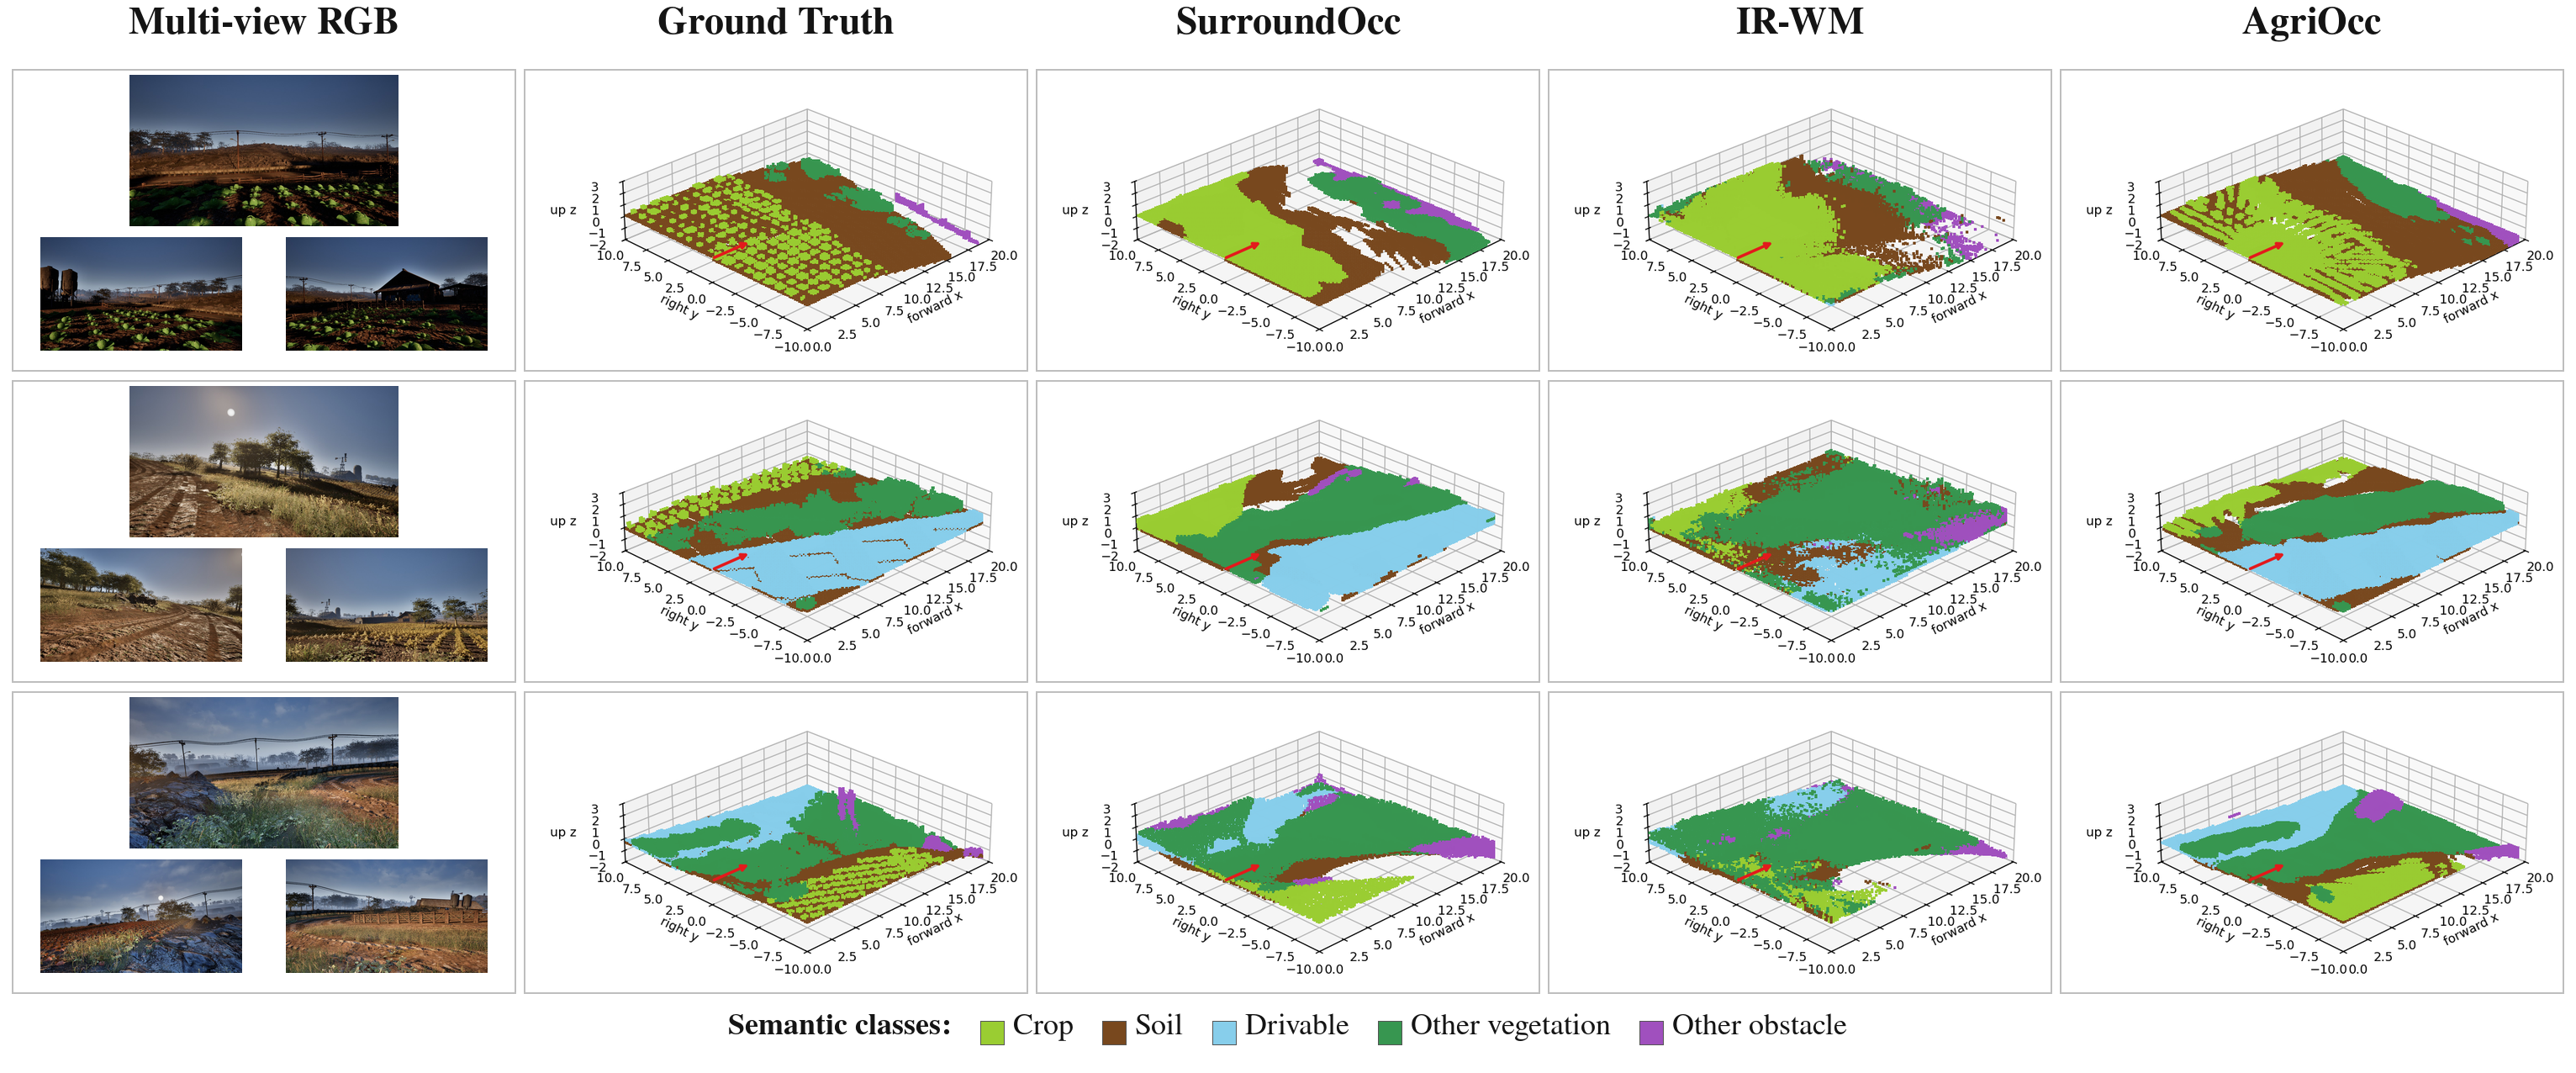
\includegraphics[width=\linewidth]{figures/qualitative_comparison_3x5.png}
\caption{AgriOcc-Dataset 上的定性比较。每一行对应一个不同作物、光照和场景条件下的样本；从左至右依次为三路输入 RGB 图像、真值标签、SurroundOcc、IR-WM 和 AgriOcc 的当前帧三维语义占用预测。}
\label{fig:qualitative_comparison}
\end{figure}

\subsection{消融实验}\label{sec:ablation}
表\ref{tab:ablation}按模块的累积方式验证各设计的作用。
GVAD 带来主要增益，表明以可见锚点约束 BEV 查询能够缓解农业场景中由遮挡和视角变化引起的几何歧义。
在此基础上，NearFar 通过将查询预算优先分配给近场区域取得进一步改善，
说明任务受益于与机器人作业范围相匹配的空间采样布局。
再加上Agri-AMoE后的完整 AgriOcc 的结果进一步表明，Agri-AMoE 与几何编码、近远场查询互补：
前者自适应选择三维局部与上下文表征，后两者提供稳定的 BEV 输入。

NearFar 的计算收益还体现为训练吞吐与显存占用。添加NearFar后训练时间相比Base+GVAD减少 10.1\%，
每卡 batch size 为 2时，峰值显存减少 29.5\%.
这说明远场稀疏查询降低了每个有效 batch 的总体编码开销，并允许使用更大的微批。


\begin{table}[htbp]
\centering
\caption{AgriOcc-Dataset 消融实验。\checkmark 表示对应模块启用。训练时间由第 8 轮平均迭代时间与每轮迭代数估算；所有配置均采用 4 张 RTX 4090 和有效全局 batch size 为 24。显存为固定每卡 batch size 为 2、一次预热后前向--反向传播测得的单卡峰值分配显存；NearFar 的显存收益与同一 GVAD--ADHR 稠密对照组比较。}
\label{tab:ablation}
\fontsize{9}{11}\selectfont
\setlength{\tabcolsep}{1.4pt}
\begin{tabular}{lccccccr}
\toprule
配置 & GVAD & NearFar & Agri-AMoE & 参数(M) & 显存(GB) & 训练(min/epoch) & mIoU(\%) \\
\midrule
Base  &  &  &  & 52.12 & 13.08 & 26.02 & 53.89 \\
+ GVAD & \checkmark &  &  & 55.08 & 15.14 & 42.93 & 56.24 \\
+ NearFar & \checkmark & \checkmark &  & 55.12 & \textbf{10.68} & 39.28 & 56.49 \\
+ Agri-AMoE & \checkmark & \checkmark & \checkmark & \textbf{55.74} & 11.03 & 40.95 & \textbf{56.99} \\
\bottomrule
\end{tabular}
\end{table}

\subsection{仿真到真实越野场景迁移}\label{sec:sim2real}
为了进一步验证仿真数据集上训练的模型在真实世界的有效性，本节我们在 ORAD-3D 数据集上
对 AgriOcc-Dataset上训练好的AgriOcc checkpoint 进行迁移学习，并评估在其官方测试集和农田子集上的性能。
ORAD-3D 的占用预测的网格形状为 $100\times100\times16$ ，共有九类体素，类别定义沿用其官方标注协议；
AgriOcc-Dataset 与 ORAD-3D 的类别和相机数不同，
因而先将 AgriOcc-Dataset checkpoint 中形状兼容的张量加载到 ORAD 模型；
三相机 embedding 取中心前视 embedding，并替换预测指定网格形状和类别的占用头，
再用ORAD 训练集进行对齐训练。

我们对比了使用ORAD-3D训练集的不同比例（10\%、25\%、50\%和100\%）进行迁移学习的结果，并与从头训练的结果进行比较。
表\ref{tab:orad}同时给出 ORAD-3D 官方测试集和从中筛选出的农田场景子集的结果。
\texttt{Test} 与 \texttt{Test (w/o Free)} 均在完整官方测试清单上计算，\texttt{Test\_farm} 则按农田子集中出现的类别计算。
为与 ORAD-3D 论文中的语义 mIoU 保持可比，表中额外报告去除 Free 类后的 Test mIoU。
结果表明，当ORAD-3D的训练集比例达到25\%和50\%时，性能已逐步接近从头训练；
当比例达到100\%时，则超过从头训练，且训练时间远低于从头训练。
可见，在AgriOcc的预训练权重上用少量真实数据进行迁移学习能够有效增强真实野外和农田场景的占用预测效果。
因此，仿真农业 occupancy 数据不仅可以用于模型研究，还能提供可迁移的三维环境表征先验，降低真实农业和越野数据需求。

\begin{table}[htbp]
\centering
\caption{ORAD-3D 仿真到真实迁移结果（\%）。\texttt{Test} 为包含 Free 类的九类平均 IoU，\texttt{Test (w/o Free)} 为仅对八个非 Free 语义类求平均的 mIoU，因而可与 ORAD-3D 论文中的结果直接比较；\texttt{Test\_farm} 为农田场景子集上按出现类别计算的 mIoU。OpenOcc、OccFormer 和 SurroundOcc 的结果引自 ORAD-3D 论文\cite{chen2025orad3d}，未报告训练时间、包含 Free 类的平均值或农田子集结果。}
\label{tab:orad}
\fontsize{9}{11}\selectfont
\setlength{\tabcolsep}{2.6pt}
\begin{tabular}{lrrrrr}
\toprule 
训练方式 & 比例 & 训练时间(min) & Test & Test (w/o Free) & Test\_farm \\
\midrule
OpenOcc从头训练 & 100% & -- & -- & 5.83 & -- \\
OccFormer从头训练 & 100% & -- & -- & 7.45 & -- \\
SurroundOcc从头训练 & 100% & -- & -- & 7.60 & -- \\
\midrule
AgriOcc从头训练 & 100\% & 54.1 & 18.16 & 9.01 & 31.83 \\
\midrule
AgriOcc迁移学习 & 10\% & 4.0 & 14.33 & 4.97 & 22.29 \\
AgriOcc迁移学习 & 25\% & 6.7 & 14.96 & 5.65 & 28.64 \\
AgriOcc迁移学习 & 50\% & 10.6 & 15.70 & 6.29 & 34.52 \\
AgriOcc迁移学习 & 100\% & 18.5 & \textbf{20.11} & \textbf{11.17} & 39.45 \\
\bottomrule
\end{tabular}
\end{table}

图\ref{fig:orad_qualitative}进一步在三个 ORAD-3D 官方测试样本上比较真值、从头训练和使用全部 ORAD-3D 训练数据迁移后的预测结果。
\begin{figure}[t]
\centering
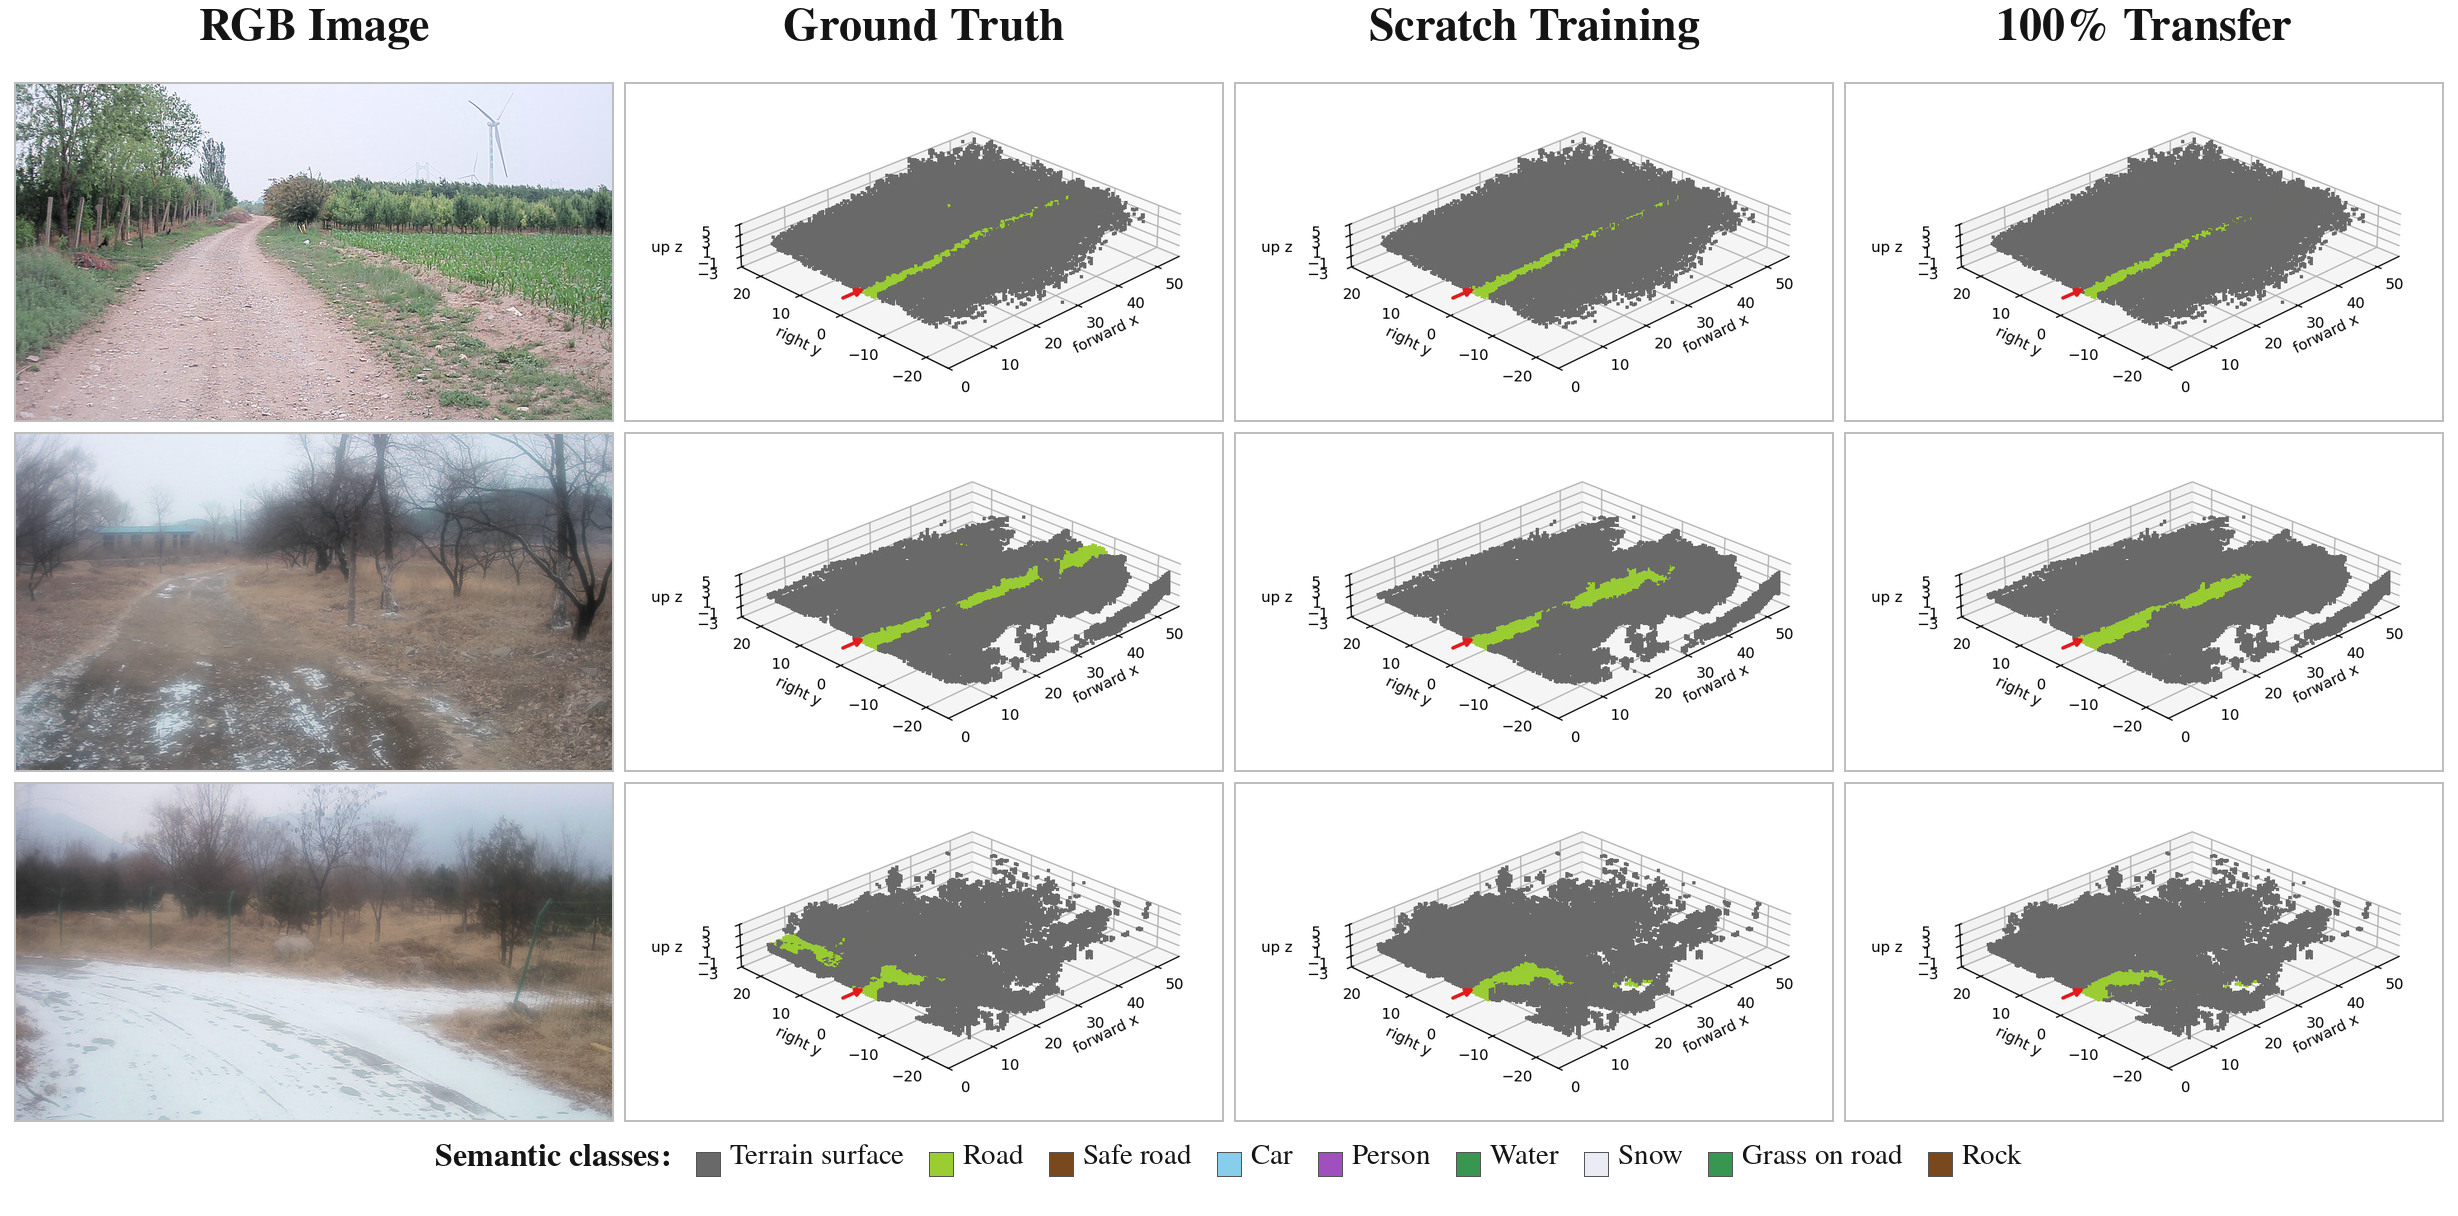
\includegraphics[width=\linewidth]{figures/orad3d_transfer_qualitative.png}
\caption{ORAD-3D 上的定性迁移比较。每行对应同一官方测试样本；从左至右为输入 RGB 图像、真值标签、使用全部 ORAD-3D 训练数据的从头训练结果，以及 AgriOcc-Dataset 预训练后在全部 ORAD-3D 训练数据上迁移的结果（100\% Transfer）。}
\label{fig:orad_qualitative}
\end{figure}

\subsection{体素分辨率迁移}\label{sec:resolution_transfer}
本文构建的AgriOcc-Dataset的体素分辨率为0.2m，与主流汽车自动驾驶语义占用基准一致\cite{behley2019semantickitti,li2024sscbench}。
但是农业机器人在垄间通行、株间避障和精细作业时，$0.2\times0.2\times0.2\,$m 的体素可能将相邻作物、
窄垄沟或局部可通行边界量化到同一网格中，带来潜在的精度不足问题。
然而，将整个 BEV 编码器直接扩展到 $0.1\times0.1\times0.2\,$m 会使
 XY 查询数从 $100\times100$ 增至 $200\times200$，即增加四倍；
 相应地，多尺度图像--BEV 交互、BEV 中间激活和三维占用监督的计算与显存开销均显著上升。
 为此，我们收集了一个$0.1\times0.1\times0.2\,$分辨率的小型仿真数据集，
 包含19300个样本，并按1：1划分为训练和验证集。
 我们使用它来进一步验证 AgriOcc 是否能够将已学习的标准分辨率三维先验高效迁移到细分辨率占用预测。

具体地，迁移模型首先在 $0.2\times0.2\times0.2\,$m AgriOcc-Dataset 数据上完成训练，
保留其 $100\times100$ GVAD--Agri-AMoE--NearFar BEV 编码器；
随后在 $0.1\times0.1\times0.2\,$m 数据上微调，并在占用输出端加入学习式 $2\times$ 细化头。
该头将粗占用 logits 与相应的 BEV 特征投影融合，输出 $200\times200\times25$ 体素。
对照组则用 0.1 m 数据集从头训练，直接学习 $200\times200$ 的高分辨率 BEV 与占用预测。
两组结果如表\ref{tab:resolution_transfer}所示。

\begin{table}[htbp]
\centering
\caption{0.1 m体素分辨率的迁移结果（\%）。
迁移方法先在 $0.2\times0.2\times0.2\,$m 数据上训练，再适配至 $0.1\times0.1\times0.2\,$m。
对照组则用 0.1 m 数据集从头训练，直接学习 $200\times200$ 的高分辨率 BEV 与占用预测。}
\label{tab:resolution_transfer}
\fontsize{9}{11}\selectfont
\setlength{\tabcolsep}{2.4pt}
\begin{tabular}{lrrrrrrrr}
\toprule
方法 & mIoU & Free & Crop & Soil & Drivable & Other veg. & Other obs. \\
\midrule
0.1 m 从头训练 & 36.18 & 89.27 & 16.74 & 52.92 & 20.11 & 23.45 & 14.56 \\
\midrule
\textbf{0.2 m 预训练 $\rightarrow$ 0.1 m 细化} & \textbf{49.01} & \textbf{92.39} & \textbf{22.61} & \textbf{73.75} & \textbf{44.29} & \textbf{35.49} & \textbf{25.50} \\
\bottomrule
\end{tabular}
\end{table}

表\ref{tab:resolution_transfer}显示，预训练迁移在所有语义类别上均优于直接高分辨率训练，
且对地面和可通行区域等连续结构的改善尤为明显。这说明 $0.2\,$m 预训练学习到了
可复用的图像--BEV 投影关系、可见性约束与场景级语义布局。
因而，微调阶段可以将有限的高分辨率监督集中用于恢复局部边界、垄沟与作物间隙，
而不必重新估计相机几何和大范围田间结构。

从优化角度看，直接高分辨率训练必须同时学习四倍数量的 BEV 查询及其图像对应关系；
在训练样本规模不变时，每个高分辨率体素获得的有效几何观测更稀疏，
迁移方案保留 $100\times100$ 编码器的稳定全局上下文，并以残差式 $2\times$ 输出细化将粗预测上采样到 0.1 m 网格。
因而，细化头只需学习粗网格未表达的高频空间残差，而不必重建完整的三维场景；
这解释了其在作物、地面和可通行区域上的一致增益，也说明 AgriOcc 能在不承担端到端高分辨率 BEV 编码成本的条件下适配精细农业感知需求。

\subsection{讨论与局限性分析}\label{sec:discussion}
AgriOcc 的总体增益集中于地面、可通行区域和复杂背景类别，说明可见性建模、
三维结构自适应解码和近远场计算分配能够提升农业场景的大范围空间一致性。
Agri-AMoE 通过梯度能量在平面局部、垂直和大范围上下文专家之间逐体素路由；
NearFar 将近场分辨率优先级显式编码到查询布局中，为农业机器人部署中的精细感知与高效计算提供了统一设计。

模型对作物细粒度结构的恢复仍存在局限。对于植株和叶片密集分布的区域，
相邻植株容易发生语义混合，模型倾向于将连续植被预测为一大片连通作物区域，因而难以保留单株间隔和细小的垄间空隙。
对于苗期等体积很小的作物，有限的图像像素和有效占据体素会使弱视觉证据在图像--BEV 投影与语义解码中被背景吸收，
图\ref{fig:limitations}展示了这些现象：卷心菜样本中真值中的株间空隙在预测中被明显填平，而早期玉米和马铃薯样本中的稀疏小尺度作物仅被部分恢复。
因此，AgriOcc 更适用于以场景级三维语义理解、通行性评估和作业安全决策为核心的农业机器人应用，
例如田间作业、果园巡检、温室移动、牧场巡逻与农场运输；对于依赖单株定位、株间距测量和精细长势评估的株级监测任务，仍存在局限。
\begin{figure}[t]
\centering
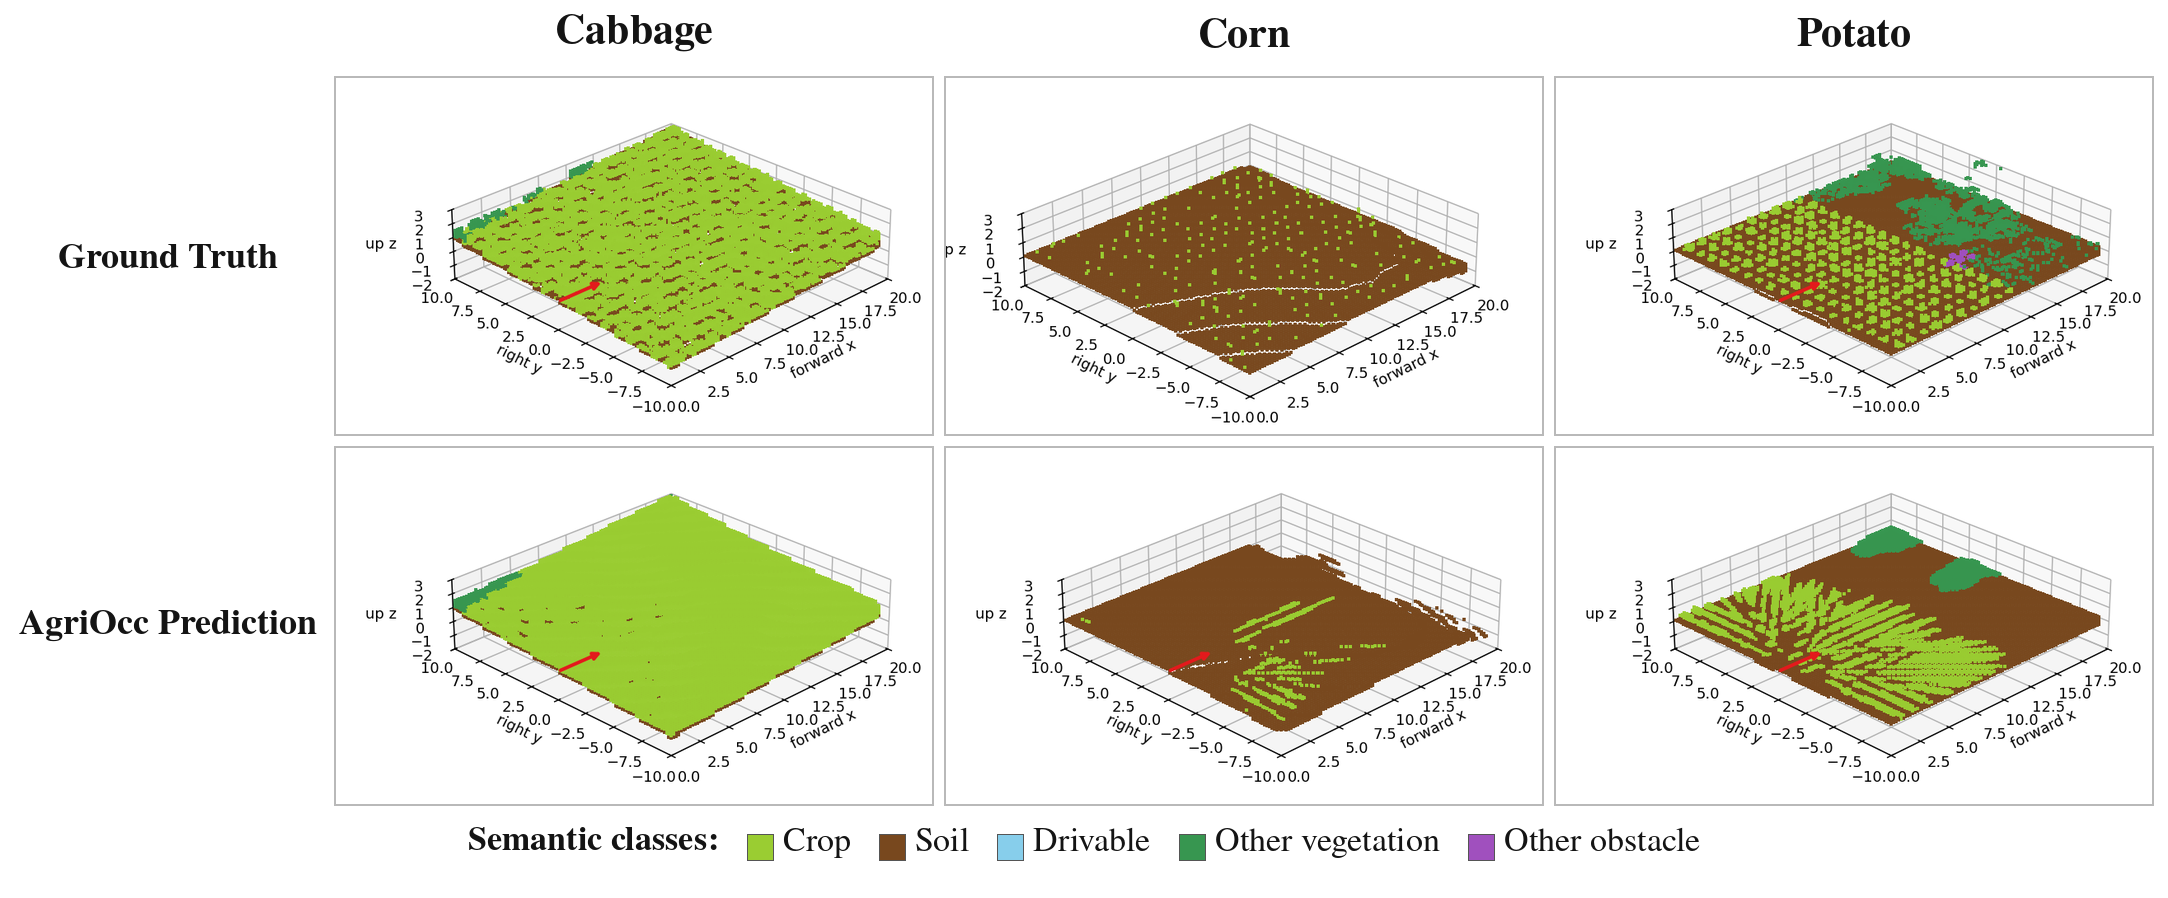
\includegraphics[width=\linewidth]{figures/farmsim_limitations_2x3.png}
\caption{AgriOcc-Dataset 上的局限性示例。第一行为真值标签，第二行为对应的 AgriOcc 预测；三列从左至右分别为卷心菜、玉米和马铃薯场景。密集作物的株间间隙易被预测为连通区域，而苗期等小尺度作物容易出现漏检或范围不足。}
\label{fig:limitations}
\end{figure}
